% 0 = resource relative path
% 1 = sample box declarations
% 2 = document body

\documentclass [11pt, a4paper, oneside, notitlepage] {article}

\usepackage[a4paper, margin=2cm]{geometry}
\usepackage[T2A]{fontenc}
\usepackage[utf8]{inputenc}
\usepackage[ukrainian, english]{babel}
\usepackage[intlimits]{amsmath}
\usepackage{amsthm}
\usepackage{amssymb}
\usepackage{float}
\usepackage{tabularx}
\usepackage{indentfirst}
\usepackage{subcaption}
\usepackage{hyperref}
\usepackage{graphicx}
\graphicspath{ {/algotester/bin/resources/} }

\allowdisplaybreaks
\widowpenalty=4774
\clubpenalty=4774

\newcolumntype{C}{>{\arraybackslash}X}

\newsavebox\boxi
\newsavebox\boxo


\begin {document}

\section*{Interesting proteins}
\hspace{1cm}
\emph{Limits: 2 sec., 512 MiB}
\bigskip

Its a known fact that the most important component of human body, it is basically the building material of every cell in your body. They are usually divided into two groups: simple and complex. But few know that there are one more but not popular classification, that divides proteins into interesting and uninteresting one.

Proteins can be represented as a set of $mathbf{N}$ nodes, where some pairs of nodes are connected with aminoacids. The proteins are always connected, thich means there is at least one sequence of connections between any two distinct pairs of nodes.

A ring in a protein is a sequence of no less than 3 nodes, in which adjacent nodes connected with aminoacids and ends of the sequence connected too.

Protein is called interesting if any node lies lies on at most one ring. An example of interesing protein is shown in the picture below:

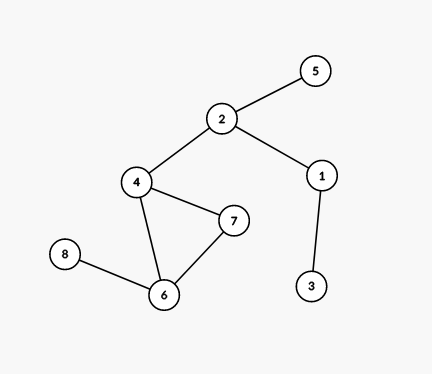
\includegraphics{interesting_graph}

To help with better understanding of interesting proteins, you were asked to answer several queries -- will the original protein be interesing after adding connection between $u_i$ and $v_i$.

\section*{Input}

The first line of input contains two integers $mathbf{N}$ and $mathbf{M}$, where $mathbf{N}$ is the number of nodes in the protein and $\mathbf{M}$ is the number of connections between nodes.

Next $\mathbf{M}$ lines contains description of connections. $i^{th}$ connections is represented by two distinct integers $u_i$ and $v_i$, which is nodes that it joins.

This is followed by line with a single integers $\mathbf{Q}$, which is the number of queries.

Following $\mathbf{Q}$ lines describe queries. Each query contains two integers $a_j$ and $b_j$ -- nodes that need to be connected to obtain graph for $j^{th}$ query.

It is guaranteed that input represents correct tree, and each for each query with nodes $a_j$ and $b_j$ there is no connection between nodes.

\section*{Output}

For each query output "Yes", if, when adding an connection between nodes $a_j$ and $b_j$, the protein remains interesting, and "No" otherwise.

\section*{Constraints}
$3 \le \mathbf{N} \le 2 * 10^5$,
$2 \le \mathbf{M} \le 2 * 10^5$,
$0 \le \mathbf{Q} \le 2 * 10^5$,
$1 \le a_j, b_j \le 2 * 10^5$,
$1 \le v_j, u_j \le 2 * 10^5$

\begin{lrbox}{\boxi}
\begin{minipage}[t]{0.5\textwidth}
\noindent
\vspace{-7mm}
\begin{verbatim}
8 8
1 2
1 3
2 4
2 5
4 6
4 7
6 8
6 7
5
3 5
2 3
5 6
1 4
7 8
\end{verbatim}
\vspace{0mm}
\end{minipage}
\end{lrbox}
\begin{lrbox}{\boxo}
\begin{minipage}[t]{0.5\textwidth}
\noindent
\vspace{-7mm}
\begin{verbatim}
Yes
Yes
No
No
No
\end{verbatim}
\vspace{0mm}
\end{minipage}
\end{lrbox}
\section*{Samples}
\begin{table}[H]
\begin{tabularx}{\textwidth}{|C|C|}
\hline
Input (\emph{stdin}) & Output (\emph{stdout}) \tabularnewline
\hline
\usebox\boxi & \usebox\boxo \tabularnewline
\hline

\end{tabularx}
\end{table}


\clearpage



\end {document}


